\section{Input Control}

The input control interface acquires an inbound frame from the Network
Interface and stores it in an internal buffer. A FSM determines
whether the inbound packet is for the device (destination IP address
matches) and if it is: 

\begin{itemize}
\item An inbound event packet
\item An inbound data retransmission request
\item An ARP Who-Has query for us
\item A ping packet. 
\end{itemize}

It then triggers the correct packet transmission module and provides
that module exclusive access to its internal buffer.


\subsection{Interface}
To acquire a frame from the NIC \signal{NEXTFRAME} is asserted; the
deassertion of \signal{DINEN} indicates the complete reception of a
packet.

The assertion of, for example, \signal{PINGSTART} tells the ICMP Echo
Reply processing module that the frame stored within should be
processed. \signal{PINGADDR[9:0]} now can access any of the 2048
stored words, which appear on \signal{PKTDATA[15:0]} one cycle later
(the standard BlockRAM latency). The processing module asserts
\signal{PINGDONE} to indicate that it has finished its processing,
allowing the acquisition of another inbound frame.

The operation of the other \signal{RETXSTART}, \signal{ARPSTART}, and
\signal{EVENTSTART} interfaces are analogous.

\subsection{Implementation} 

We use a dual-ported BlockRAM as a packet storage buffer, and read in
the frame into the buffer. The FSM then examines the contents of the
frame by setting \signal{INTADDRB} to various values and decoding the
results.

\begin{itemize}
\item \textbf{ARP Query} : The FSM checks Ethernet Protocol type and
  ARP query type.
\item \textbf{ICMP Echo Request}: The FSM checks Ethernet Protocol
  type, IP protocol type, and ICMP meaning fields.
\item \textbf{Retransmission Request} : The FSM checks Ethernet
  Protocol type, IP protocol type, and port number.
\item \textbf{Inbound events} : The FSM checks Ethernet Protocol type,
  IP protocol type, and port number.
\end{itemize}

Packet analysis begins in \signal{NONE}, and terminates in the
\signal{NEXTPKT} state, the latter repeated in Figure
\ref{inputcontrol.fsm} for clarity.

\begin{figure}
\begin{centering}
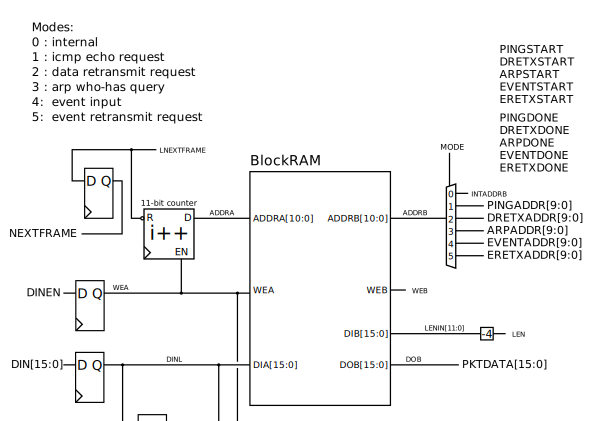
\includegraphics[scale=0.8]{inputcontrol.svg}
\end{centering}
\caption{Input control implementation.}
\label{inputcontrol}
\end{figure}

\begin{figure}
\begin{centering}
\includegraphics[scale=0.8]{inputcontrol.fsm.svg}
\end{centering}
\caption{Input Control FSM. Note that the termiating \signal{NEXTPKT} state is repeated for the purpose of clarity. }
\label{inputcontrol.fsm}
\end{figure}


